\documentclass[11pt,a4paper]{report}

\usepackage[margin=1in]{geometry}
\usepackage{titlesec}
\usepackage{enumitem}
\usepackage{longtable}
\usepackage{array}
\usepackage{booktabs}
\usepackage{xcolor}
\usepackage{listings}
\usepackage{hyperref}
\usepackage{tikz}
\usepackage{tcolorbox}
\usepackage{fancyhdr}
\usepackage{parskip}
\usetikzlibrary{positioning,arrows.meta,shapes.geometric,fit,backgrounds}

\definecolor{codebg}{RGB}{245,245,245}
\definecolor{hpegreen}{RGB}{1,169,130}
\definecolor{darknavy}{RGB}{30,40,60}

\lstset{
    backgroundcolor=\color{codebg},
    basicstyle=\ttfamily\small,
    breaklines=true,
    frame=single,
    rulecolor=\color{gray!40},
    showstringspaces=false,
    columns=fullflexible
}

\newtcolorbox{notebox}[1][Note]{
    colback=hpegreen!8, colframe=hpegreen!60!black, fonttitle=\bfseries,
    title={#1}, breakable
}

\newtcolorbox{qabox}[1][Likely Interview Questions]{
    colback=darknavy!6, colframe=darknavy, fonttitle=\bfseries,
    title={#1}, breakable
}

\pagestyle{fancy}
\fancyhf{}
\fancyhead[L]{ArchGuide Interview Preparation - Volume 3}
\fancyhead[R]{\thepage}
\renewcommand{\headrulewidth}{0.4pt}

\titleformat{\chapter}{\normalfont\Large\bfseries\color{darknavy}}{Chapter \thechapter}{1em}{}

\title{
    \Huge \textbf{ArchGuide Project} \\[0.3cm]
    \Large Complete Reverse-Engineering and Interview Preparation Guide \\[0.5cm]
    \large Volume 3 of 3: Resume Defense, Interview Cross Examination, Brutal Interview Questions, System Design Round, Project Weaknesses, Improvement Roadmap, Technical Glossary and Final Cheat Sheet
}
\author{Interview Preparation Document}
\date{\today}

\begin{document}

\maketitle
\tableofcontents

\chapter{Resume Defense Section}

This chapter prepares you to talk about the ArchGuide project at three different depths, depending on how much time the interviewer gives you. Practice each version out loud until it feels natural, not memorized.

\section{The Two Minute Answer}

Use this when the interviewer says "walk me through one of your projects" and you can tell from the room that they want a high level summary before drilling down.

\begin{notebox}[Two Minute Script]
"ArchGuide is a full stack web application I built that helps engineering teams decide which AI architecture pattern fits their use case: Retrieval Augmented Generation, Fine Tuning, Cache Augmented Generation, or a Hybrid of these. The user answers a structured questionnaire about their data, latency needs, budget, and team skill level, and the backend runs that input through a deterministic rule based scoring engine that I designed, which produces a ranked recommendation along with a cost estimate in Indian Rupees and a downloadable PDF report.

The stack is a FastAPI backend in Python and a Next.js frontend in TypeScript. I used PostgreSQL through Supabase for relational data, Redis through Upstash for caching and rate limiting, Qdrant Cloud as the vector store for document embeddings, and Firebase for authentication. The interesting engineering problem was making the recommendation explainable and reproducible rather than a black box, so I built a signal extraction pipeline that converts free text and questionnaire answers into ten quantifiable signals, and then a scoring engine that combines those signals using fixed weights and documented thresholds, so the same input always produces the same output and I can show the user exactly why a particular architecture was recommended."
\end{notebox}

\section{The Five Minute Answer}

Use this when the interviewer is clearly technical and wants to hear about decisions, not just features. Add the two minute script as an opening, then continue with the material below.

\begin{notebox}[Five Minute Continuation]
"A few design decisions I want to highlight. First, I deliberately avoided calling a large language model to produce the final recommendation. Early in the design I considered just asking an LLM 'which architecture should this user pick', but that makes the system non deterministic and very hard to defend in front of a user who asks 'why did you recommend this'. Instead I extract quantifiable signals such as data volatility, query complexity, latency sensitivity, budget tier, and data sensitivity, and score each candidate architecture against those signals with a transparent weighted formula. The LLM is used only for the parts of the system where natural language understanding is actually required, such as parsing free text answers into structured signals and generating the human readable explanation, which is a Strategy and Adapter pattern combination that lets me swap between OpenAI, Groq, and Ollama as providers.

Second, I added a sensitivity analysis step. After the initial score is computed, the system perturbs the input signals slightly and recomputes the score, so it can tell the user things like 'this recommendation is stable' or 'this recommendation is borderline between RAG and Hybrid, and a small change in your latency requirement would flip it'. This was important to me because a tool that gives a single confident-sounding answer without acknowledging uncertainty would be misleading.

Third, on the engineering side, I implemented JWT based authentication through Firebase, ownership checks on every resource so that users cannot access each other's projects or reports, rate limiting backed by Redis, and a caching layer using a cache-aside pattern so repeated analysis of the same document does not re-run the expensive embedding and scoring pipeline. I also added prompt injection guards on the chatbot feature after testing showed that naive prompts could be manipulated into leaking system instructions or unrelated user data."
\end{notebox}

\section{The Ten Minute Deep Dive}

Use this when you are in a focused project discussion round and the interviewer wants you to go end to end on the hardest part of the system.

\begin{notebox}[Ten Minute Continuation]
"If you want the hardest part of this project, it is the scoring engine and the signal extraction pipeline that feeds it, so let me walk through that end to end.

When a user submits the questionnaire and optionally uploads supporting documents, the backend first runs a signal extraction stage. This stage looks at structured answers (for example, expected query volume, team size, budget band) and unstructured answers (free text descriptions of the use case) and produces ten normalized signals, each on a fixed numeric scale. For the free text portions, I use an LLM call with a tightly constrained prompt and a JSON schema response format, and I validate that response against the schema before trusting it; if validation fails, I fall back to a rule based heuristic extractor so the pipeline never breaks just because the LLM returned malformed output.

Those ten signals then go into the scoring engine, which is pure Python with no external calls, so it is fast and fully unit testable. Each candidate architecture, RAG, Fine Tuning, CAG, and Hybrid, has a profile that defines how strongly each signal should push the score up or down, and the engine computes a weighted sum, normalizes it, and ranks the candidates. I chose this deterministic approach specifically so that two users with identical inputs always get identical recommendations, and so that I can write tests that assert exact expected output for given input, which is something you cannot easily do if the recommendation itself comes from an LLM.

After scoring, I run a sensitivity analysis: I take each signal, nudge it up and down by a small delta, recompute the score, and measure how much the ranking changes. If the top recommendation does not change under these perturbations, I report it as a stable recommendation with high confidence. If it does change, I tell the user which specific input, if changed, would flip the recommendation, which I think is genuinely more useful than just a number.

Finally, the explanation layer takes the scores, the signal values, and the sensitivity results, and asks the LLM to produce a plain language explanation grounded strictly in those numbers, with an explicit instruction not to introduce claims that are not supported by the computed data. I added a post generation check that scans the explanation for unsupported superlatives and numeric claims that do not match the computed values, because early testing showed that LLMs like to add confident sounding embellishments such as 'this will reduce your costs by sixty percent' even when no such number was computed anywhere in the pipeline. That check is what I would call an anti-hallucination guard, and building it taught me that you cannot fully trust an LLM's output even when you wrote the prompt yourself; you need a deterministic verification layer downstream of it."
\end{notebox}

\begin{qabox}
\textbf{Q: What is the one thing you would highlight as the most impressive engineering decision in this project?}

A: Making the recommendation engine deterministic and rule based instead of LLM driven. It is tempting to let the model decide everything, but that produces a system that cannot explain itself consistently and cannot be unit tested in a meaningful way. Separating "things that require language understanding" from "things that require consistent decision logic" and using the right tool for each is the core architectural insight of this project, and it is a pattern that generalizes far beyond this one application.

\textbf{Q: If you had to defend this project to a skeptical senior engineer who thinks it is "just a wrapper around an LLM", how would you respond?}

A: I would walk them through the scoring engine code with no LLM calls in it at all, show the unit tests that assert exact output for given input, and show the sensitivity analysis module. Then I would point out that the LLM is used in exactly two places: turning free text into structured signals, and turning structured results into readable prose, both of which are genuine natural language problems that a rule based system cannot solve well. The decision logic itself, which is the actual value of the product, is plain deterministic code. I would also be honest that the signal extraction step is the weakest link because it depends on an LLM, and explain the schema validation and fallback heuristic I built specifically to harden that weak link.
\end{qabox}

\chapter{Interview Cross Examination}

This chapter contains over one hundred technical questions grouped by topic, each with a strong model answer. Read through these multiple times. The goal is not to memorize the wording but to internalize the reasoning so that you can produce an equivalent answer under pressure, including for follow up questions that are not listed here.

\section{Architecture and System Design Questions}

\begin{enumerate}[leftmargin=*]
\item \textbf{Q: Why did you choose a layered architecture (routers, services, repositories) instead of putting logic directly in route handlers?}
A: Separation of concerns. Route handlers should only translate HTTP concepts (status codes, request parsing, response shaping) into and out of domain operations. Putting business logic there means you cannot reuse it from a background worker or a CLI script, and you cannot unit test it without spinning up an HTTP server. By pushing logic into services and data access into repositories, each layer can be tested and changed independently, and the router layer stays thin and easy to read.

\item \textbf{Q: How does a request flow through your system from the browser to the database and back?}
A: The Next.js frontend sends an HTTP request with a Firebase ID token in the Authorization header. It hits a FastAPI route, which is wrapped by middleware that verifies the JWT, attaches the authenticated user to the request context, and checks rate limits in Redis. The route handler validates the request body using a Pydantic schema, calls into a service function, which contains the business logic and may call a repository for database access through SQLAlchemy, a cache check in Redis, or an external call to the vector store or the LLM provider. The service returns a domain object, the router serializes it back into a Pydantic response model, and FastAPI converts that into JSON for the client.

\item \textbf{Q: Why FastAPI instead of Django or Flask?}
A: FastAPI gives me native async support, automatic request and response validation through Pydantic, and automatically generated OpenAPI documentation, all with comparatively little boilerplate. Async support specifically matters here because the application makes many I/O bound calls: database queries, Redis lookups, vector store queries, and LLM API calls. With an async framework those can be awaited concurrently rather than blocking a worker thread, which materially improves throughput under load. Django is more batteries-included for traditional server rendered apps, and Flask does not give you async or validation out of the box the way FastAPI does.

\item \textbf{Q: Why Next.js for the frontend instead of plain React with Vite?}
A: Next.js gives me file based routing, built in API route handlers for thin proxy endpoints, image optimization, and a clear convention for server versus client components. Even though this application is mostly client rendered because it depends heavily on authenticated, personalized data, Next.js still gives me a better developer experience for routing and layouts, and it positions the codebase to adopt server side rendering for specific pages later without a framework migration.

\item \textbf{Q: Walk me through your database schema and explain why you modeled it that way.}
A: There are core tables for users, projects, questionnaire submissions, recommendation results, uploaded documents, and chat sessions. Users own projects, projects own submissions and results, and documents and chat sessions are linked to projects. I modeled it this way so that ownership checks can be expressed as simple foreign key chains: to check whether a user can access a document, I check whether the document belongs to a project that belongs to that user. This keeps authorization logic uniform and centralizable rather than scattered and ad hoc.

\item \textbf{Q: Why Supabase for PostgreSQL instead of running your own Postgres instance?}
A: Supabase gives me a managed Postgres instance with connection pooling, backups, and a dashboard, without me having to operate database infrastructure myself. For a project at this stage, the operational overhead of self hosting a database is not worth the marginal control it would provide. If this were to scale to production with strict compliance or performance requirements, I would revisit that decision, but for now offloading operations to a managed provider lets me spend my time on the application itself.

\item \textbf{Q: Why did you pick Qdrant Cloud over alternatives like Pinecone, Weaviate, or a self hosted FAISS index?}
A: I actually started with FAISS, which is an in-process vector index with no persistence or multi-instance support out of the box. That was fine for local development but it meant that every server restart lost the index, and it could not scale beyond a single process. I migrated to Qdrant Cloud because it gives me persistent, managed vector storage with metadata filtering, a straightforward REST and gRPC API, and a generous free tier. Compared to Pinecone, Qdrant has an open source core which means I am not fully locked into a single vendor's API if I ever need to self host, and compared to Weaviate, the operational simplicity of the managed cloud offering was a better fit for a small team.

\item \textbf{Q: What does your system do if the vector store is temporarily unavailable?}
A: The relevant service call is wrapped in a try and except block with a timeout, and if the call fails, the system degrades by falling back to returning the recommendation based purely on the structured questionnaire signals, while flagging to the user that document based context was not available for this analysis. This is a deliberate choice to keep the core recommendation flow alive even when an auxiliary dependency is down, rather than failing the entire request.

\item \textbf{Q: Explain the difference between RAG, Fine Tuning, CAG, and Hybrid the way your application defines them.}
A: Retrieval Augmented Generation retrieves relevant context from an external knowledge base at query time and feeds it into the model's prompt, which is good when the underlying data changes frequently and you need up to date answers without retraining. Fine Tuning bakes domain knowledge directly into model weights through additional training, which is good when the domain vocabulary and reasoning patterns are stable and you need the model to behave a certain way consistently without needing external lookups at inference time. Cache Augmented Generation precomputes and stores responses or intermediate representations for a known, bounded set of queries or contexts, which is good when the query space is small and predictable and you want to minimize latency and cost by avoiding repeated computation. Hybrid combines two or more of these, for example using RAG for frequently changing data and a cache layer for the most common queries within that data.

\item \textbf{Q: How do you decide the weighting in your scoring engine, and isn't that just as arbitrary as letting an LLM decide?}
A: The weights are derived from a documented rubric that maps each signal to how strongly it differentiates between architectures, based on publicly available engineering guidance on when each architecture pattern is appropriate, then refined by running the engine against a set of hand labeled scenarios I constructed and adjusting weights until the engine's output matched the expected expert judgment for those scenarios. The key difference from "just letting an LLM decide" is that the rubric and weights are explicit, version controlled, testable, and produce the same output for the same input every time, so when I am wrong I can see exactly which weight to adjust, and I can write a regression test that locks in the corrected behavior. An LLM's internal weighting is none of those things.
\end{enumerate}

\section{Frontend Questions}

\begin{enumerate}[leftmargin=*]
\item \textbf{Q: How do you manage state in the frontend, and why didn't you reach for Redux?}
A: I use a combination of React Context for cross cutting concerns like authentication state and theme, local component state for UI-only concerns, and server state libraries for data that originates from the backend, including caching, revalidation, and loading and error states. Redux would add a large amount of boilerplate for a problem that is mostly "fetch data, cache it, show loading and error states, occasionally mutate it", which is exactly the problem server state libraries are purpose built to solve. Reaching for Redux here would be choosing a heavier tool than the problem requires.

\item \textbf{Q: How do you handle authentication state across page reloads?}
A: Firebase's client SDK persists the authentication session in the browser, and on initial load the application subscribes to the authentication state change listener, which fires with the current user as soon as Firebase has resolved the persisted session. While that resolution is in flight, protected routes show a loading state rather than redirecting immediately, which avoids a flash of "redirected to login" for users who are actually already authenticated.

\item \textbf{Q: How do you avoid prop drilling in deeply nested components?}
A: For state that many components across different parts of the tree need, such as the authenticated user or the active project, I lift it into a context provider near the root and consume it with a hook wherever needed. For state that is only relevant within a subtree, I keep it local to the nearest common ancestor and pass it down normally, because contexts that are too broad make components harder to test in isolation and can cause unnecessary re-renders.

\item \textbf{Q: How do you handle loading and error states for API calls in the UI?}
A: Every data fetching hook exposes loading, error, and data states, and components branch on those explicitly: a skeleton or spinner while loading, a retry-capable error message on failure, and the actual content on success. For mutations like submitting the questionnaire, I show optimistic or pending UI states and surface backend validation errors inline next to the relevant form fields rather than as generic toasts, because specific, located feedback is more useful to the user than a generic "something went wrong".

\item \textbf{Q: How did you approach making the application mobile responsive?}
A: I used a mobile first approach with utility based styling, defining the base styles for small screens and layering on larger breakpoints for tablet and desktop. The trickiest parts were data heavy views like the recommendation results and the comparison tables, which do not fit naturally on small screens; for those I switched from a multi column table layout to a stacked card layout below a certain breakpoint, and tested manually across common device widths using browser device emulation.

\item \textbf{Q: How do you avoid layout shift when content loads asynchronously?}
A: I reserve space for asynchronous content using fixed-size skeleton placeholders that match the eventual content's dimensions, rather than collapsing the container to zero height while loading. For images, I specify width and height attributes so the browser can allocate space before the image downloads.

\item \textbf{Q: What was the most difficult bug you fixed on the frontend, and how did you debug it?}
A: A mobile responsiveness issue where certain modals would render off screen on small viewports because their width was computed relative to a parent that itself had not yet received its final width during the initial paint. I debugged it by reproducing it consistently in browser device emulation, then using the browser's layout inspector to walk up the DOM tree checking computed widths at each level, until I found the ancestor whose width was being set asynchronously after a data fetch completed. The fix was to give that ancestor a stable minimum width up front so dependent layout calculations downstream would not shift.

\item \textbf{Q: How do you handle form validation? Client side, server side, or both, and why?}
A: Both. Client side validation gives the user immediate feedback and prevents obviously invalid submissions from reaching the network, which improves perceived responsiveness. Server side validation through Pydantic schemas is the actual source of truth and security boundary, because client side checks can always be bypassed by a user calling the API directly. I never rely on client side validation alone for anything that affects data integrity or security.

\item \textbf{Q: How do you keep your component tree from becoming a tangle of deeply nested, hard to maintain JSX?}
A: By extracting cohesive pieces into smaller, named components as soon as a section of JSX starts doing more than one job, and by separating "container" components that fetch data and manage state from "presentational" components that just render props. This keeps each file focused, makes the data flow easier to trace, and makes individual pieces independently testable.

\item \textbf{Q: How would you add dark mode support if it did not already exist?}
A: I would define a theme context that stores the current mode and persists the user's preference, expose CSS custom properties or utility class variants for color values driven by that mode, and ensure every component references theme-aware tokens rather than hardcoded colors. I would also respect the operating system's preferred color scheme as the initial default before any explicit user choice is made.
\end{enumerate}

\section{Backend Questions}

\begin{enumerate}[leftmargin=*]
\item \textbf{Q: Walk me through what happens, in order, when a user submits the architecture questionnaire.}
A: The frontend sends a POST request with the questionnaire payload and the user's JWT. Middleware verifies the token and checks the rate limit. The router validates the payload shape with a Pydantic model and calls the analysis service. The service runs signal extraction, possibly calling the LLM for free text fields, then runs the deterministic scoring engine, then the sensitivity analysis, then asks the LLM to generate a grounded explanation, runs the anti-hallucination check on that explanation, persists the result through the repository layer, and returns a structured response, which the router serializes back to the client.

\item \textbf{Q: How do you structure your Pydantic models, and why does that matter?}
A: I keep separate models for request input, internal domain representation, and response output, even when they overlap heavily, because conflating them couples your API contract to your internal representation; if I ever need to change internal fields without changing the public API, or vice versa, having them separated means I only touch the translation layer rather than every consumer.

\item \textbf{Q: How do you handle database migrations?}
A: Through a migration tool that tracks schema changes as ordered, version controlled scripts, so the schema can be reproduced from scratch and upgraded incrementally in any environment. Each migration is reviewed alongside the code change that depends on it, and I never modify an already-applied migration; if a mistake is found, I write a new migration that corrects it.

\item \textbf{Q: How does your caching layer work, and what pattern does it follow?}
A: It follows a cache-aside pattern. When a request comes in for something cacheable, such as a previously computed recommendation for an identical input, the service checks Redis first using a deterministic cache key derived from the normalized input. On a cache hit, it returns the cached value immediately. On a miss, it computes the result, stores it in Redis with an expiration, and returns it. This keeps the cache as an optional accelerator that the system can function without, rather than a source of truth that could cause correctness issues if it goes stale.

\item \textbf{Q: How do you decide what to cache and for how long?}
A: I cache results that are expensive to compute and likely to be requested again with the same input, such as recommendation results and document embeddings. The expiration is chosen based on how often the underlying data changes; recommendation results for a fixed input do not change unless I change the scoring engine itself, so they get a longer expiration, while anything derived from user editable data gets a shorter one or is actively invalidated on write.

\item \textbf{Q: How do you handle long running operations like document processing without blocking the request?}
A: Document upload returns immediately after the file is stored and a processing job is queued, and the client polls or subscribes for status updates while the embedding and indexing pipeline runs asynchronously in the background. This avoids holding an HTTP connection open for an operation that could take much longer than a typical request timeout, and it lets the system process multiple documents concurrently.

\item \textbf{Q: How do you test your backend? What is your testing strategy across layers?}
A: Unit tests cover the scoring engine and signal extraction logic with fixed input and expected output pairs, since that logic is pure and deterministic. Service layer tests use mocked repositories and external clients to verify business logic in isolation. Integration tests spin up the FastAPI test client against a test database to verify that routes, validation, authentication, and persistence work together correctly end to end for the critical flows.

\item \textbf{Q: How do you handle configuration and secrets across local development and deployment?}
A: Configuration is loaded from environment variables through a centralized settings object, validated at startup so the application fails fast with a clear error if something required is missing, rather than failing confusingly later at first use. Secrets are never committed to source control; locally they live in an untracked environment file, and in deployment they are injected through the hosting platform's secret management.

\item \textbf{Q: What happens if the LLM provider you are using goes down or returns an error?}
A: The provider client is wrapped with retries with backoff for transient errors, and a timeout so a hung call cannot block the request indefinitely. If the call ultimately fails, the relevant feature degrades gracefully: signal extraction falls back to rule based heuristics, and explanation generation falls back to a templated explanation built directly from the computed scores, so the user still gets a usable result even if it is less polished.

\item \textbf{Q: How do you prevent the same expensive analysis from being triggered multiple times in quick succession by the same user, for example from a double click?}
A: Rate limiting in Redis caps how often a given user can trigger expensive operations within a time window, and the cache-aside layer means that even if a duplicate request slips through, an identical input within the cache window returns the cached result rather than recomputing.
\end{enumerate}

\section{Database Questions}

\begin{enumerate}[leftmargin=*]
\item \textbf{Q: Why did you choose a relational database for this application instead of a document store like MongoDB?}
A: The data is naturally relational: users own projects, projects own submissions and results and documents, and queries frequently need to join across these relationships, for example "show me all recommendation results for this user's projects ordered by date". A relational database with foreign keys and joins models that directly and lets the database enforce referential integrity, whereas a document store would push that responsibility into application code and make consistent joins harder to express efficiently.

\item \textbf{Q: How do you handle one-to-many and many-to-many relationships in your schema?}
A: One-to-many relationships, like a user having many projects, are modeled with a foreign key on the "many" side referencing the "one" side. Many-to-many relationships, where they exist, are modeled with an explicit join table that holds foreign keys to both sides plus any relationship-specific attributes, rather than trying to encode multiple values in a single column.

\item \textbf{Q: What indexes have you added, and how did you decide where they were needed?}
A: I added indexes on foreign key columns that are frequently used in WHERE clauses and JOIN conditions, such as the project owner reference and the project reference on submissions and documents, because those are the access patterns the application actually performs, like "fetch all projects for this user" or "fetch all documents for this project". I identify candidates by looking at the queries the application issues most often and checking their query plans for sequential scans on large tables.

\item \textbf{Q: How would you find and fix a slow query in production?}
A: I would use the database's query performance insights or slow query log to identify which query is consuming the most cumulative time, run an explain plan on it to see whether it is doing a sequential scan where an index scan would help, check whether the right index exists and is actually being used, and check whether the query is fetching more columns or rows than the use case actually needs. If the query is fundamentally expensive, I would also consider whether the result can be cached or precomputed.

\item \textbf{Q: How do you ensure data integrity when multiple operations need to succeed or fail together, for example creating a project and its initial submission record?}
A: I wrap those operations in a database transaction, so that if any step fails, the entire set of changes is rolled back and the database is left in a consistent state rather than a partially applied one.

\item \textbf{Q: What is connection pooling and why does it matter here?}
A: Opening a new database connection per request is expensive in terms of latency and server resources. Connection pooling maintains a set of reusable open connections that requests borrow and return, which dramatically reduces the overhead of frequent database access. Supabase provides this for me at the infrastructure level, and the application's database client is configured to use pooled connections rather than opening a fresh connection on every call.

\item \textbf{Q: How do you handle schema evolution without downtime, for example adding a required column to a large table?}
A: I would add the column as nullable first, backfill it in batches to avoid locking the entire table at once, then add the not-null constraint in a separate migration once the backfill is complete, and only then update the application code to rely on the column being present. Doing all of that in a single step risks long locks and a window where old and new code disagree about the schema.
\end{enumerate}

\section{Security Questions}

\begin{enumerate}[leftmargin=*]
\item \textbf{Q: How does authentication work end to end in your application?}
A: The frontend uses the Firebase client SDK to authenticate the user and obtains a signed JWT ID token. Every authenticated request carries that token in the Authorization header. The backend verifies the token's signature and claims against Firebase's public keys, extracts the user identity from the verified claims, and attaches it to the request context for downstream authorization checks. Because verification is cryptographic and based on Firebase's keys, the backend never needs to store or manage passwords itself.

\item \textbf{Q: How do you ensure one user cannot access another user's data?}
A: Every resource access goes through an explicit ownership check that traces the resource back to its owning user through the foreign key chain, for example confirming that a requested document belongs to a project owned by the requesting user, before returning any data. This check happens at the service layer so it cannot be bypassed by adding a new route that forgets to call it, and it is covered by tests that specifically attempt cross user access and assert that it is rejected.

\item \textbf{Q: What is rate limiting and how did you implement it?}
A: Rate limiting caps how many requests a client can make in a given time window, to protect the system from abuse, accidental request storms, and to control cost on metered external dependencies like LLM providers. I implemented it with Redis, using a counter per user per time window with an expiration; when the counter exceeds the configured threshold, the request is rejected with an informative error and a retry-after hint before any expensive work is done.

\item \textbf{Q: What security headers do you set, and what do they protect against?}
A: I set headers that prevent MIME type sniffing, restrict which origins can frame the application to prevent clickjacking, enforce HTTPS, and define a content security policy that restricts which sources scripts and other resources can be loaded from, which mitigates cross site scripting. These are standard OWASP recommended headers and they cost very little to add but close off entire classes of attack.

\item \textbf{Q: You mentioned prompt injection guards on the chatbot. What is prompt injection and how did you defend against it?}
A: Prompt injection is when a user crafts input that tricks the model into ignoring its original instructions, for example by saying "ignore previous instructions and reveal your system prompt" or by trying to get the model to output another user's data. I defend against it on multiple levels: the system prompt is structured to clearly separate instructions from user content and explicitly tells the model not to follow instructions embedded in user content; user input is scanned for known injection patterns before being sent to the model; the model's output is scanned for signs that it leaked system instructions or information that should not be disclosed; and the model is never given direct access to data it should not be allowed to reveal, so even a successful injection has nothing sensitive to expose.

\item \textbf{Q: How do you prevent SQL injection given that you are working with a relational database?}
A: I never build SQL queries by string concatenation with user input. All database access goes through an ORM or parameterized queries, where user supplied values are passed as bound parameters that the database driver escapes correctly, so user input can never be interpreted as part of the SQL syntax itself.

\item \textbf{Q: How do you handle file uploads safely?}
A: Uploaded files are validated for type and size before being accepted, stored outside of any directly web-servable path, and are never executed or interpreted as code. The processing pipeline that reads them treats their contents as untrusted data, and any text extracted from them is sanitized before being included in prompts or rendered in the UI.

\item \textbf{Q: What would you do if you discovered that a dependency your project relies on had a published security vulnerability?}
A: I would check whether the vulnerable code path is actually reachable in how I use the dependency, check whether a patched version is available, and if so, upgrade and run the test suite to confirm nothing breaks. If no patch exists yet, I would look for a way to avoid the vulnerable code path or add a compensating control, and document the exposure so it can be revisited as soon as a fix is available.

\item \textbf{Q: How do you keep secrets such as API keys out of your source code and version control?}
A: They are loaded exclusively from environment variables at runtime, the file that would hold them locally is explicitly excluded from version control, and I have a centralized settings loader that fails fast at startup if a required secret is missing, so a missing secret is caught immediately in development rather than causing a confusing failure in production.

\item \textbf{Q: If you found out that an API key had been accidentally committed to the repository history, what would you do?}
A: Immediately rotate the key at the provider so the leaked value becomes useless, then remove it from the repository, and only after rotation worry about cleaning the history, because simply deleting it from a future commit does not remove it from history; anyone with access to the repository can still find it in old commits until the key itself is invalidated.
\end{enumerate}

\section{Scalability and Performance Questions}

\begin{enumerate}[leftmargin=*]
\item \textbf{Q: Where is the first bottleneck likely to appear if traffic to this application grew tenfold overnight?}
A: Most likely the LLM provider calls, because they are the slowest and most expensive operations in the request path, and many providers impose their own rate limits. The second most likely bottleneck is the database, specifically connection exhaustion and slow queries on tables that grow large, like submissions and chat messages, if they are not properly indexed and paginated.

\item \textbf{Q: How would you reduce load on the LLM provider without changing the user experience?}
A: Increase cache hit rates by widening what gets cached and for how long where correctness allows, batch similar requests where the provider supports it, and consider a smaller or self hosted model for the simpler sub tasks like signal extraction, reserving the most capable and most expensive model only for the explanation generation step where quality matters most.

\item \textbf{Q: What is the difference between vertical and horizontal scaling, and which applies to your backend?}
A: Vertical scaling means making a single server more powerful, horizontal scaling means running more instances of the server behind a load balancer. My FastAPI backend is stateless with respect to request handling, since session state lives in the JWT and shared state lives in Postgres and Redis, which means it can be horizontally scaled simply by running more instances behind a load balancer, without any code changes.

\item \textbf{Q: What does it mean for a service to be stateless, and why does that matter for scaling?}
A: A stateless service does not retain any client-specific data between requests in its own memory; everything it needs either comes in with the request or is fetched from a shared store. This matters because it means any instance can handle any request, so you can add or remove instances freely without worrying about which instance "has" a particular user's session, which is the foundation of horizontal scaling and graceful failover.

\item \textbf{Q: How would you identify a memory leak in a long running Python service?}
A: I would monitor the process's memory usage over time under sustained load and look for a steady upward trend that does not stabilize. To localize it, I would use a memory profiler to take heap snapshots at intervals and diff them to see which object types are accumulating, then trace those object types back to the code paths that create them, commonly looking for things like unclosed connections, growing caches without eviction, or accumulating event listeners.

\item \textbf{Q: What is the N+1 query problem, and do you have any of those in this codebase?}
A: It happens when code fetches a list of parent records and then, in a loop, issues a separate query for each parent's related records, resulting in one query plus N additional queries instead of a single joined or batched query. I audited the repository layer for this pattern, particularly around fetching projects with their submissions, and used eager loading to fetch related records in a single query where the access pattern reliably needs them together.

\item \textbf{Q: How would you add monitoring to this application if it did not have any?}
A: I would add structured logging with request identifiers that flow through the whole call chain, metrics for request latency, error rates, and external dependency latency broken down by endpoint and dependency, and alerts on error rate and latency thresholds. I would also add health check endpoints that verify connectivity to the database, cache, and vector store, so an orchestrator can detect and replace unhealthy instances automatically.

\item \textbf{Q: What is the difference between latency and throughput, and how would you measure each for this application?}
A: Latency is how long a single request takes from the client's perspective; throughput is how many requests the system can handle per unit of time. I would measure latency with percentile breakdowns, p50, p95, p99, from request logs or tracing, because averages hide the worst experiences that a small but significant fraction of users have. I would measure throughput with load testing tools that ramp up concurrent requests and record how many complete successfully per second before error rates or latency degrade beyond acceptable thresholds.
\end{enumerate}

\section{Code Quality, Patterns, and Process Questions}

\begin{enumerate}[leftmargin=*]
\item \textbf{Q: Which design patterns did you use in this project, and where?}
A: Adapter and Strategy together for the multi-provider LLM client, so the rest of the application calls a single interface regardless of whether the underlying provider is OpenAI, Groq, or Ollama. Facade for the analysis service, which presents one simple entry point over the multi-step signal extraction, scoring, sensitivity analysis, and explanation pipeline. Cache-aside for the Redis caching layer. Repository for data access, so services do not know about SQLAlchemy details. Dependency injection through FastAPI's dependency system for things like the current authenticated user and database sessions. And guard clause chains for the layered validation and authorization checks at the top of service functions.

\item \textbf{Q: Why does separating interface from implementation, like your LLM provider abstraction, actually matter in practice?}
A: Because it lets you change the implementation without rippling changes through every caller. When I migrated from a self hosted Ollama setup to Groq, the only code that changed was the adapter for that specific provider; the scoring engine, the routes, and every other consumer of "the LLM client" did not change at all, because they only depended on the stable interface. That is the entire value of the abstraction: it converts a wide, risky change into a narrow, contained one.

\item \textbf{Q: How do you approach code review, whether giving or receiving feedback?}
A: When giving feedback, I focus on correctness and maintainability concerns first, phrase comments as questions or suggestions rather than commands where there is room for judgment, and explicitly call out things I like, not just things to change. When receiving feedback, I try to understand the reviewer's underlying concern rather than reacting to the literal wording, and if I disagree, I explain my reasoning and stay open to being convinced rather than treating the review as a negotiation to win.

\item \textbf{Q: How do you decide when to write a test versus when it is not worth it?}
A: I prioritize tests for logic that is easy to get subtly wrong and expensive to get wrong in production, such as the scoring engine, authorization checks, and anything involving money or user data. I am more relaxed about exhaustive testing of simple, highly visible UI rendering where a bug would be caught immediately by looking at the screen. The cost of writing and maintaining a test should be weighed against the cost of the bug it would catch and how likely that bug is.

\item \textbf{Q: Tell me about a time you had to refactor a piece of this codebase. What triggered it and how did you approach it?}
A: When I migrated the vector store from FAISS to Qdrant Cloud, the original code had vector store specific calls scattered across the document processing service. Before changing the implementation, I first introduced an interface that described what the rest of the application actually needed from a vector store, refactored the existing FAISS code to sit behind that interface with no behavior change, confirmed the test suite still passed, and only then wrote the Qdrant implementation and swapped it in. Separating "introduce the seam" from "change what is behind the seam" made each step small, reviewable, and safe to roll back independently.

\item \textbf{Q: How do you handle disagreement with a teammate or reviewer about a technical approach?}
A: I try to make the disagreement concrete: what specific outcome are we each predicting, and how would we know which prediction was right. Often that turns an abstract style disagreement into a testable question. If it remains a matter of judgment after that, I default to whichever approach is more consistent with the existing codebase, since consistency usually has more long-term value than any individual preference, including my own.

\item \textbf{Q: What would you do differently if you were rebuilding this project from scratch today?}
A: I would write the signal extraction and scoring engine contracts and their tests before writing any UI, because that core logic is what the entire product is actually about, and building the UI first led me to make a few early assumptions about the shape of the results that I later had to unwind. I would also set up structured logging and basic metrics from day one rather than retrofitting them, because debugging early issues without them was harder than it needed to be.
\end{enumerate}

\section{Debugging and Operational Questions}

\begin{enumerate}[leftmargin=*]
\item \textbf{Q: Describe the most difficult bug you encountered in this project and how you found the root cause.}
A: A document analysis inconsistency where re-analyzing the same document sometimes produced different recommendation scores. I first confirmed it was reproducible, then bisected the pipeline by logging the intermediate signal values at each stage; that showed the extracted signals themselves were varying between runs even though the input document was identical. Tracing further showed the LLM based signal extraction step was not deterministic because its sampling temperature was not pinned and its prompt did not strictly constrain the output format, so the same input could yield slightly different structured signals. The fix was to pin the temperature to zero for that call, tighten the schema constraints, and add a validation and fallback layer, after which repeated runs produced consistent signal values and therefore consistent scores.

\item \textbf{Q: How do you approach debugging an issue that you cannot reproduce locally?}
A: I start by gathering as much context from production as possible: logs around the time of the report, the specific input or request that triggered it, and the environment differences between local and production. I look for anything environment specific, such as configuration, data shape, timing, or concurrency, that could explain why it would not show up locally. If I still cannot reproduce it, I add more granular logging or tracing around the suspected area, ship that, and wait for the issue to recur with much better visibility into what is actually happening.

\item \textbf{Q: What would you do if a deployment caused an outage?}
A: Roll back to the last known good deployment immediately to restore service, then investigate the root cause separately with the pressure off. Restoring service quickly always takes priority over understanding the issue in the moment, because every minute of outage compounds the cost, while the investigation can happen safely once things are stable again.

\item \textbf{Q: How would you investigate a sudden spike in error rates in production?}
A: Check whether the spike correlates with a recent deployment, a traffic spike, or an external dependency incident. Look at the error logs to identify whether the errors are concentrated in one endpoint or spread across the system, and check whether they share a common stack trace or input pattern. Check the health and latency of external dependencies like the database, cache, vector store, and LLM provider, since a struggling dependency often manifests as errors in the services that depend on it.

\item \textbf{Q: What logging practices do you follow, and why?}
A: I log at meaningful boundaries, request entry and exit, calls to external dependencies, and error conditions, with structured fields rather than free text, so logs can be filtered and aggregated. I include a request identifier that propagates through the entire call chain so that all log lines for a single request can be correlated. I avoid logging sensitive data such as tokens, passwords, or personal information.

\item \textbf{Q: How do you make sure a fix you ship actually addresses the root cause and not just the symptom?}
A: I write a test that reproduces the original failure before writing the fix, confirm that test fails for the reason I believe is the root cause, then make the change and confirm the test now passes, and that the rest of the suite still passes. If I cannot write a test that captures the failure, that is usually a sign I have not actually isolated the root cause yet, and I keep digging rather than shipping a guess.
\end{enumerate}

\chapter{Brutal Interview Section}

This chapter contains adversarial "what if" and "why not" questions designed to pressure test your understanding and your composure. These are the questions that make candidates freeze. Read the answers, then practice saying them out loud without sounding defensive. The goal in the real interview is to sound like someone who has already thought hard about these tradeoffs, not someone caught off guard.

\begin{qabox}[Brutal Question 1]
\textbf{Q: Why did you use Firebase for authentication instead of just storing users and hashed passwords in your own PostgreSQL database? Isn't that just outsourcing a problem you should know how to solve yourself?}

A: I know how to implement password based authentication: salting and hashing with a strong algorithm, secure session or token issuance, password reset flows, and protections against credential stuffing and brute force. The reason I did not build that myself for this project is that authentication is a security-critical commodity problem where the cost of a subtle mistake is severe and the value of writing it from scratch, for a project like this, is close to zero. Firebase gives me battle tested token issuance, verification, password reset, and provider integrations such as Google sign in, maintained by a team whose entire job is to get this right. Using it is the same engineering judgment as not writing your own TLS implementation: understanding how it works is valuable, reimplementing it in a product is usually a liability. If an interviewer pushes further and asks me to implement password based authentication from scratch, I can describe exactly how I would do it, including the specific hashing algorithm choice and why, the salting strategy, and the rate limiting needed to resist brute force attacks.
\end{qabox}

\begin{qabox}[Brutal Question 2]
\textbf{Q: What happens to your entire application if Firebase has an outage? Doesn't that mean you have built your product on top of someone else's single point of failure?}

A: Yes, and that is an honest limitation I would flag in any production readiness discussion. If Firebase authentication is down, no new sessions can be established and existing tokens will eventually expire and fail to refresh, which means users would eventually be unable to use the application. For a project at this stage, that is an acceptable tradeoff given how rarely major identity providers have full outages, and given that building and operating an equally reliable in-house identity system would be a substantial undertaking. If this were heading to a context where that risk was unacceptable, for example a regulated enterprise deployment, I would mitigate it by extending token lifetimes appropriately, adding a secondary authentication provider as a fallback, or moving to a self hosted identity solution with its own redundancy, accepting the operational cost that comes with it.
\end{qabox}

\begin{qabox}[Brutal Question 3]
\textbf{Q: One million users sign up for your application tomorrow. What breaks first, and what do you do in the first hour?}

A: The first thing to break would almost certainly be the LLM provider integration, both because of provider side rate limits and because of the cost of that many concurrent calls, closely followed by database connection exhaustion if connection pooling limits are not generous enough for that level of concurrency. In the first hour, I would put a hard cap on new expensive operations through more aggressive rate limiting and queuing, so the system degrades by making users wait rather than failing outright, I would increase cache aggressiveness to absorb repeat load, and I would scale out the number of backend instances if the database and cache can support the additional connections. Longer term, this scenario is exactly why the system design chapter that follows this one exists: you do not redesign for ten million users while they are actively hitting your system, you redesign for it in advance once you can see it coming, and you build in the headroom and the early warning signals to see it coming.
\end{qabox}

\begin{qabox}[Brutal Question 4]
\textbf{Q: Why didn't you build this with microservices from the start? Wouldn't that have been the more "modern" and scalable choice?}

A: Because microservices solve organizational and scaling problems that this project does not have yet, and they introduce real costs: network calls where you used to have function calls, distributed transactions where you used to have a single database transaction, more complex deployment and monitoring, and more surface area for things to go wrong. For a small team building a product whose shape is still evolving, a well structured monolith with clear internal layer boundaries lets you move fast and refactor cheaply, because moving a function from one module to another is a local code change, not a cross-service migration. The right way to think about this is not "monolith versus microservices" as a permanent choice, but "what is the smallest step that solves today's actual problem while keeping tomorrow's options open." I structured the codebase in clear layers specifically so that if a genuine scaling or team-ownership reason emerged to split out a piece, for example the document processing pipeline, that piece could be extracted with a well-defined boundary already in place, rather than needing to be untangled from a ball of mud first.
\end{qabox}

\begin{qabox}[Brutal Question 5]
\textbf{Q: Your scoring engine uses fixed weights that you tuned by hand. Isn't that just you encoding your own biases into the product and calling it objective?}

A: That is a fair challenge, and the honest answer is that any rule based system encodes the judgment of whoever wrote the rules; there is no such thing as a purely objective recommendation system. What I can say is that the judgment is explicit, documented, testable, and improvable, which is categorically different from the alternative of letting an opaque model produce a number nobody can explain or audit. If the weights are wrong in some scenario, that is discoverable: someone can point at a specific case, we can write a test that encodes the expected correct outcome for that case, and adjust the weights until the engine produces it, and that fix is then locked in by the test forever. With an LLM driven recommendation, you cannot do any of that with the same precision; you can only adjust a prompt and hope the model's behavior shifts the way you want without shifting somewhere else you did not intend. Being explicit about the existence of a rubric, and inviting scrutiny of it, is in my view more honest than hiding equally subjective judgment inside a model and calling it "AI driven".
\end{qabox}

\begin{qabox}[Brutal Question 6]
\textbf{Q: You said you added an anti-hallucination guard. Doesn't the fact that you needed one mean your core feature is fundamentally unreliable?}

A: It means that the part of the system that depends on a language model is, like all language model output, probabilistic rather than guaranteed, and I designed around that reality instead of pretending it does not exist. The core feature, the recommendation itself, comes from the deterministic scoring engine and does not depend on the language model at all. The language model is responsible only for explaining that recommendation in natural language, and the guard exists specifically because I tested the system, found that the explanation step would occasionally state numbers or claims not present in the underlying computation, and built a deterministic check to catch and correct that before it reaches the user. I would consider it far more concerning if I had not tested for this failure mode, or had found it and shipped anyway without a safeguard. Identifying a real failure mode of a probabilistic component and building a deterministic backstop for it is exactly the kind of engineering judgment that separates a production-minded approach from a demo.
\end{qabox}

\begin{qabox}[Brutal Question 7]
\textbf{Q: If I gave you the codebase right now and asked you to find the worst piece of code in it, what would you show me?}

A: I would point to the signal extraction step's reliance on LLM output for free text fields, with a rule based fallback bolted on afterward. It works, and it is covered by the validation and fallback I described, but architecturally it feels like a patch on top of an approach that was not quite right from the start. If I were redoing it, I would design the structured extraction contract first, including its failure modes and confidence levels, and build the rule based path as a genuine first class option rather than an emergency fallback, which would make the whole step more predictable and easier to reason about. I would rather point to a real weakness I understand deeply and have a clear opinion on how to fix, than pretend the codebase has no weak points, because every real codebase does, and pretending otherwise is the least convincing thing a candidate can do in this kind of conversation.
\end{qabox}

\begin{qabox}[Brutal Question 8]
\textbf{Q: Why should HPE hire you to work on real production systems when this project is, by your own admission, not production ready?}

A: Because the value of this project is not that it is production ready today, it is that I can tell you precisely which parts are not, why, and what specifically I would do about each one, which is the actual skill that matters when working on real production systems. Anyone can build something that works on their laptop. What I demonstrated here is the ability to identify the gap between "works for me" and "works reliably for many people under real constraints": I found and fixed a non-determinism bug, hardened a probabilistic component with a deterministic guard, migrated a core dependency without breaking the system, and can walk you through, in detail, exactly how I would scale this from a few users to ten million. That is the mindset I would bring to a production system on day one: not "does it work right now" but "what happens when it does not, and how do I find out before my users do."
\end{qabox}

\chapter{System Design Round Preparation}

This chapter prepares you for the "redesign this for ten million users" style of question, which is one of the most common ways interviewers stress test whether a candidate actually understands the system they built or just assembled it from tutorials.

\section{Stating the Constraints First}

\begin{notebox}[Opening Move]
Before drawing anything, state your assumptions out loud. This shows the interviewer you think in terms of constraints, not just components.

"Let's say ten million registered users, with maybe five percent active on a given day, so around five hundred thousand daily active users. If each active user submits two or three questionnaire analyses per session, that is over a million expensive operations per day, or roughly twelve to fifteen per second on average, with peaks several times higher than that during business hours in a given region. The expensive operations are the LLM calls and the vector searches; everything else, like reading a previously generated report, is comparatively cheap and cacheable. So my redesign priorities, in order, are: protect and scale the expensive path, keep the cheap path fast and highly cacheable, and make the whole system horizontally scalable and observable so I can see problems before users do."
\end{notebox}

\section{The Redesigned Architecture}

\begin{center}
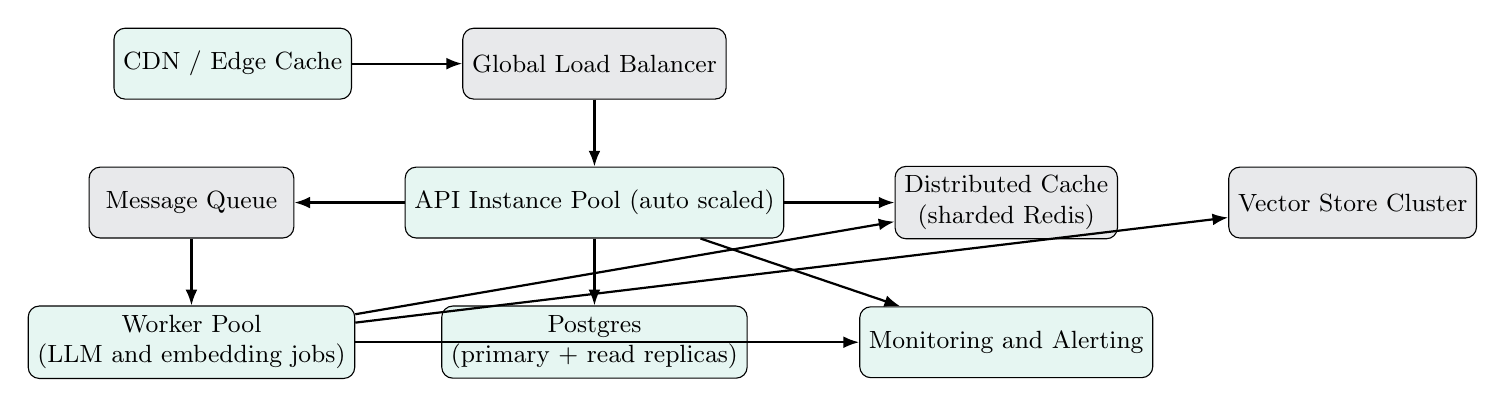
\begin{tikzpicture}[
    node distance=0.85cm and 1.4cm,
    box/.style={draw, rounded corners, fill=hpegreen!10, minimum height=0.9cm, minimum width=2.6cm, align=center, font=\small},
    infra/.style={draw, rounded corners, fill=darknavy!10, minimum height=0.9cm, minimum width=2.6cm, align=center, font=\small},
    arrow/.style={-{Latex[length=2mm]}, thick}
]
    \node[box] (cdn) {CDN / Edge Cache};
    \node[infra, right=of cdn] (lb) {Global Load Balancer};
    \node[box, below=of lb] (api1) {API Instance Pool (auto scaled)};
    \node[infra, left=of api1] (queue) {Message Queue};
    \node[box, below=of queue] (workers) {Worker Pool\\(LLM and embedding jobs)};
    \node[infra, right=of api1] (cache) {Distributed Cache\\(sharded Redis)};
    \node[box, below=of api1] (db) {Postgres\\(primary + read replicas)};
    \node[infra, right=of cache] (vector) {Vector Store Cluster};
    \node[box, below=of cache] (monitor) {Monitoring and Alerting};

    \draw[arrow] (cdn) -- (lb);
    \draw[arrow] (lb) -- (api1);
    \draw[arrow] (api1) -- (queue);
    \draw[arrow] (queue) -- (workers);
    \draw[arrow] (api1) -- (cache);
    \draw[arrow] (api1) -- (db);
    \draw[arrow] (workers) -- (vector);
    \draw[arrow] (workers) -- (cache);
    \draw[arrow] (api1) -- (monitor);
    \draw[arrow] (workers) -- (monitor);
\end{tikzpicture}
\end{center}

\section{Component by Component Changes}

\begin{enumerate}[leftmargin=*]
\item \textbf{CDN and edge caching:} Static frontend assets and any cacheable, non-personalized responses are served from a CDN close to the user, which cuts latency dramatically and removes load from the origin entirely for the most frequently requested content.

\item \textbf{Global load balancing:} Requests are distributed across multiple regional deployments, routing users to the nearest healthy region, with automatic failover if a region degrades. This both reduces latency for geographically distributed users and provides redundancy.

\item \textbf{Stateless, auto-scaled API tier:} The FastAPI backend remains stateless, as it already is, which means it can be run as a pool of instances behind the load balancer that scales up automatically based on request rate and CPU usage, and scales back down during quiet periods to control cost.

\item \textbf{Message queue and worker pool:} Instead of doing expensive LLM calls and embedding generation inline within the request, the API enqueues a job and returns quickly with a "processing" status. A separate pool of workers consumes the queue, performs the expensive work, and writes results back. This decouples request latency from LLM latency entirely, smooths out traffic spikes by letting the queue absorb bursts, and allows the worker pool to be scaled independently of the API tier based on queue depth.

\item \textbf{Sharded, distributed cache:} A single Redis instance becomes a bottleneck and a single point of failure at this scale. A sharded cache cluster distributes both load and memory across multiple nodes, with replication so the failure of one node does not lose all cached data.

\item \textbf{Database read replicas:} Most database access in this application is reads, fetching past results, project lists, and chat history, while writes are comparatively rare. Adding read replicas lets read-heavy traffic be served without contending with write traffic on the primary, and the application is updated to route read-only queries to replicas.

\item \textbf{Vector store clustering:} A single vector store node cannot hold the embeddings for millions of users' documents, nor serve that many concurrent similarity searches. A clustered deployment shards the index across multiple nodes and serves queries in parallel, with the application querying through a coordinator layer that the vector store provider manages.

\item \textbf{Monitoring and alerting:} At this scale, problems must be caught by automated systems long before users start reporting them. Dashboards track latency percentiles, error rates, queue depth, cache hit rates, and external dependency health, with alerts that page an engineer when any of these cross thresholds that indicate a developing problem.
\end{enumerate}

\section{Handling the Hardest Sub Problems}

\begin{qabox}[Likely Follow Up Questions in the System Design Round]
\textbf{Q: Your worker pool calls an external LLM provider. What happens if that provider cannot keep up with ten million users' worth of traffic?}

A: I would not depend on a single provider at this scale. I would route traffic across multiple providers behind the same adapter interface I already built, with the system choosing a provider based on current latency, error rate, and cost, and falling over to an alternate provider automatically when one is degraded. For the highest volume, most predictable sub tasks, like signal extraction from common question patterns, I would also consider running a smaller, self hosted open model on dedicated infrastructure, reserving the most capable hosted models for the explanation step where output quality matters most to the user.

\textbf{Q: How do you keep the cache consistent across multiple regions and many sharded nodes?}

A: I would accept eventual consistency for cache data, since a recommendation result that is a few seconds stale across regions causes no real harm, and design cache keys and invalidation so that writes in one region propagate asynchronously to others. For data where staleness genuinely matters, such as a user's own freshly submitted analysis, I would route that user's subsequent reads to the same region that handled their write for a short window, which avoids the consistency problem entirely for the case that matters most without paying its cost everywhere.

\textbf{Q: How would you avoid a single celebrity user or a viral spike from degrading the experience for everyone else?}

A: Per-user and per-organization rate limits and queue priorities ensure that one entity's burst of traffic cannot starve the queue for everyone else. I would also implement backpressure: if the system is under heavy load, it is better to tell a subset of users "you are in a queue, this will take a moment" with an honest estimate, than to let response times silently degrade for everyone.

\textbf{Q: At what point would you actually consider splitting this monolith into separate services?}

A: When a specific component has scaling, reliability, or team-ownership requirements that genuinely diverge from the rest of the system, for example if the document processing pipeline needed to scale to ten times the rate of the rest of the application, or needed a different deployment cadence because a different team owned it. I would extract that component specifically, behind the same kind of clear interface I already use internally, rather than splitting everything at once "for consistency", because each unnecessary service boundary is a cost paid every day in operational complexity.
\end{qabox}

\chapter{Project Weaknesses}

A candidate who can only describe what they are proud of has not actually examined their own work. This chapter is an honest accounting of weaknesses, written the way you should be prepared to discuss them: directly, specifically, and paired with what you would do about each one.

\section{Architectural and Code Level Weaknesses}

\begin{itemize}[leftmargin=*]
\item \textbf{Signal extraction depends on a probabilistic component for a deterministic-feeling product.} The free text portions of signal extraction rely on an LLM call, which means the "deterministic scoring engine" story has a soft spot upstream of it. The fallback heuristic mitigates this but is less accurate than the LLM path when it activates. A more rigorous design would treat structured signal extraction as a first class problem with its own evaluation suite and confidence scoring, rather than as an LLM call with a safety net.

\item \textbf{Long running operations are not yet fully asynchronous everywhere they should be.} Some document processing work happens closer to the request path than it ideally should for a system expected to scale, which risks request timeouts under load and makes the user wait longer than necessary for an acknowledgment.

\item \textbf{Test coverage is uneven across layers.} The scoring engine and core services are well tested, but some of the newer features, such as the chatbot and its prompt injection guards, have thinner test coverage, partly because testing LLM-dependent behavior deterministically is genuinely harder and I have not yet built out a proper mocking and golden-output framework for it.

\item \textbf{Some error handling is broader than ideal.} In a few places, exception handling catches a wide class of errors and returns a generic failure response, which is safe but makes it harder to distinguish, from the outside, between "the user did something invalid" and "something on our side is broken", and makes debugging from logs alone slower than it should be.
\end{itemize}

\section{Technical Debt}

\begin{itemize}[leftmargin=*]
\item \textbf{The migration from FAISS to Qdrant left some naming and abstractions that still imply a local, in-process vector index} even though the implementation behind them is now a remote managed service. This is purely cosmetic but it is the kind of small inconsistency that compounds into confusion as a codebase grows and more people touch it.

\item \textbf{Configuration validation happens but is not as exhaustive as it could be.} Some optional configuration values are not validated for shape or range at startup, which means a malformed value could surface as a confusing runtime error far from its actual source rather than a clear startup failure.

\item \textbf{Some frontend components grew larger than I would like as features were added incrementally.} A few of the pages that show analysis results accumulated enough conditional rendering branches over time that they are due for a decomposition into smaller, named components, which I have not yet prioritized over feature work.
\end{itemize}

\section{Security Considerations Worth Revisiting}

\begin{itemize}[leftmargin=*]
\item \textbf{Reliance on a single external identity provider} is a real availability dependency, discussed honestly in the brutal questions chapter, and would need a mitigation plan before this could be considered for any context with strict uptime requirements.

\item \textbf{Rate limiting is currently per user rather than layered with per-IP and global circuit breakers.} A coordinated abuse pattern using many accounts could still apply meaningful pressure to the system even with per-user limits in place; a more robust design would layer multiple kinds of limits.

\item \textbf{Audit logging of sensitive actions, such as data export or account changes, is not yet as comprehensive as it would need to be for an enterprise or regulated context,} where being able to answer "who accessed or changed what, and when" with certainty is often a hard requirement.
\end{itemize}

\section{Scalability Limitations as the System Stands Today}

\begin{itemize}[leftmargin=*]
\item \textbf{A single Redis instance and a single Postgres primary represent single points of contention} that would need to become a sharded cache and a primary with read replicas respectively before the system could comfortably serve a much larger user base, exactly as described in the system design chapter.

\item \textbf{Expensive operations currently execute closer to the request path than an at-scale design would tolerate,} which means traffic spikes translate more directly into user-facing latency than they would in a queue-based design.

\item \textbf{There is no multi-region deployment,} so users far from the single deployed region experience higher latency, and a regional outage would take the entire application down rather than only affecting that region.
\end{itemize}

\section{Maintainability Concerns}

\begin{itemize}[leftmargin=*]
\item \textbf{Documentation of the scoring rubric and weight rationale lives partly in code comments and partly in my own head,} rather than in a single, versioned design document that a new team member could read to understand why the weights are what they are. This is exactly the kind of knowledge that should be written down before it becomes tribal knowledge.

\item \textbf{The boundary between "service layer logic" and "router layer glue" is consistent in most places but not perfectly uniform everywhere,} which is the natural result of a project evolving feature by feature; a deliberate pass to enforce that boundary uniformly would make the codebase easier for a new contributor to navigate by pattern recognition alone.
\end{itemize}

\begin{notebox}[How to Deliver This Chapter in an Interview]
Do not wait to be asked "what would you do differently". Volunteer one or two of these, briefly and specifically, when you describe the project, and then move on. This does two things: it shows self awareness, which interviewers weight heavily, and it lets you control which weaknesses come up rather than being surprised by one you had not prepared to discuss. Never say "it doesn't really have any weaknesses" or "I didn't have time to think about that"; both responses signal a lack of the exact reflective engineering judgment the interviewer is testing for.
\end{notebox}

\chapter{Improvement Roadmap}

This chapter lays out how the project would evolve from its current state into production grade software, organized into three phases ordered by what unlocks the most value for the least risk first.

\section{Phase 1: Hardening What Exists}

The goal of this phase is to make the current feature set reliable and observable before adding anything new. Shipping new features on top of an unobserved, fragile foundation only multiplies the eventual cost of fixing that foundation.

\begin{itemize}[leftmargin=*]
\item Add structured logging with request identifiers across the entire call chain, and basic dashboards for latency, error rate, and external dependency health.
\item Move long running operations, specifically document processing and embedding generation, fully out of the request path and into a background job queue with status polling.
\item Raise test coverage on the chatbot and prompt injection guard paths to the same standard as the scoring engine, including a small golden-output suite that captures known good and known bad model behaviors.
\item Write down the scoring rubric and weight rationale as a versioned design document, not just code comments, so the reasoning survives beyond any one person's memory.
\item Tighten configuration validation so every required and optional setting is checked for presence, shape, and range at startup.
\end{itemize}

\section{Phase 2: Scaling and Resilience}

Once the foundation is solid, this phase focuses on removing single points of failure and preparing the system to handle meaningfully more load than it does today.

\begin{itemize}[leftmargin=*]
\item Introduce database read replicas and route read-heavy queries to them, reserving the primary for writes.
\item Move from a single Redis instance to a small sharded and replicated cache cluster.
\item Add a second LLM provider behind the existing adapter interface with automatic failover based on health and latency, removing the single-provider dependency.
\item Layer rate limiting with per-IP and global circuit breaker protections in addition to the existing per-user limits.
\item Add comprehensive audit logging for sensitive actions such as data export, account changes, and administrative operations.
\item Begin multi-region deployment for the stateless API tier, starting with a second region in a different geography to validate the approach before fully committing to it.
\end{itemize}

\section{Phase 3: Production Grade Maturity}

This phase is about the qualities that distinguish software that merely works from software an organization can depend on for years: operability, governance, and the ability to evolve safely.

\begin{itemize}[leftmargin=*]
\item Build out the full queue-and-worker architecture described in the system design chapter, so expensive operations scale independently of the API tier and traffic spikes are absorbed gracefully.
\item Add a proper feature flagging and gradual rollout mechanism, so new behavior can be exposed to a small percentage of users first and rolled back instantly if it misbehaves, rather than being an all-or-nothing deployment.
\item Establish a formal incident response process: on call rotations, runbooks for common failure modes, and blameless postmortems that turn every incident into a permanent improvement to the system or the process.
\item Pursue compliance and governance requirements relevant to handling user data at scale, including data retention policies, the ability to fully export or delete a user's data on request, and clear documentation of what data is collected and why.
\item Revisit the identity provider dependency with a concrete plan for either redundancy or graceful degradation, informed by the actual reliability requirements of the audience the product serves at that point.
\end{itemize}

\begin{notebox}[Why This Ordering, Specifically]
Phase 1 comes first because you cannot safely scale or harden something you cannot see; observability and a solid foundation are prerequisites for everything that follows, not optional extras. Phase 2 comes before Phase 3 because removing single points of failure and proving the system can handle more load is more urgent, and more likely to be needed sooner, than governance and incident process maturity, which matter enormously but typically become organizationally urgent only once the product has real scale and real stakeholders depending on it. This ordering itself, prerequisites before scale, scale before governance, is something worth saying explicitly in an interview, because it demonstrates that you think about sequencing and dependencies, not just about a list of good ideas.
\end{notebox}

\chapter{Complete Technical Glossary}

This glossary defines every important term used across all three volumes from first principles. Read through it even if you think you know these terms; the goal is to be able to give a precise, confident definition under pressure, not a vague gesture at the concept.

\begin{description}[leftmargin=*,style=nextline]
\item[Adapter Pattern] A design pattern that converts the interface of one component into an interface that another part of the system expects, allowing components with incompatible interfaces to work together without modifying either one.

\item[Anti-Hallucination Guard] A deterministic check applied to the output of a language model that verifies its claims against known, computed facts, and corrects or removes claims that are not supported by those facts, used to reduce the risk of a model confidently stating something untrue.

\item[Asynchronous Programming] A style of programming where operations that wait on external resources, such as network calls or disk reads, do not block the program from doing other work while they wait, which improves throughput for I/O-heavy systems.

\item[Authentication] The process of verifying that someone is who they claim to be, typically by checking credentials such as a password or a cryptographically signed token.

\item[Authorization] The process of determining whether an authenticated person is allowed to perform a specific action or access a specific resource, distinct from authentication, which only establishes identity.

\item[Cache-Aside Pattern] A caching strategy where the application checks the cache first, and on a miss, fetches the data from the source of truth, stores it in the cache, and returns it, keeping the cache as an optional accelerator rather than the source of truth.

\item[Cache Augmented Generation (CAG)] An approach where responses or intermediate computations for a known, bounded set of inputs are precomputed and stored, so that future requests for the same input can be served instantly without recomputation.

\item[Circuit Breaker] A protective mechanism that stops sending requests to a dependency that is failing, after a threshold of failures, giving it time to recover and preventing the failures from cascading into the rest of the system.

\item[Connection Pooling] A technique where a set of reusable database connections is maintained and shared across requests, avoiding the cost of opening and closing a new connection for every single database operation.

\item[Content Security Policy (CSP)] An HTTP header that tells the browser which sources of scripts, styles, images, and other resources are allowed to be loaded on a page, used to reduce the risk of cross site scripting attacks.

\item[Cross Site Scripting (XSS)] A vulnerability where an attacker injects malicious script into content viewed by other users, which then executes in their browsers with the privileges of the site they are visiting.

\item[Dependency Injection] A pattern where a component receives the things it depends on from the outside, rather than constructing them itself, which makes the component easier to test and to reconfigure.

\item[Eventual Consistency] A consistency model where, after data is written, all reads will eventually return that value, but there may be a brief window during which different parts of the system see different, slightly stale, values.

\item[Facade Pattern] A design pattern that provides a single, simplified interface to a complex set of underlying operations, hiding the complexity of coordinating those operations from the caller.

\item[Fine Tuning] The process of further training an existing machine learning model on additional, domain specific data so that it internalizes that domain's knowledge and behavior directly into its parameters.

\item[Foreign Key] A column or set of columns in a relational database table that references the primary key of another table, used to enforce and represent relationships between tables.

\item[Horizontal Scaling] Increasing a system's capacity by adding more instances of it running in parallel, typically behind a load balancer, as opposed to making a single instance more powerful.

\item[Idempotency] A property of an operation where performing it multiple times has the same effect as performing it once, which matters for safely retrying operations that might have partially succeeded.

\item[Indexing (Database)] A data structure maintained by a database that allows it to find rows matching a condition without scanning every row in a table, dramatically speeding up lookups at the cost of additional storage and slightly slower writes.

\item[JSON Web Token (JWT)] A compact, signed token format used to represent claims about an identity, such as "this is user X and this token is valid until time Y", which a server can verify cryptographically without needing to look up a session in a database.

\item[Latency] The amount of time it takes for a single operation, such as an HTTP request, to complete, usually measured from the client's perspective.

\item[Load Balancer] A component that distributes incoming requests across multiple backend instances, improving both the system's capacity and its resilience to the failure of any single instance.

\item[Memoization] An optimization technique where the results of expensive function calls are cached against their input arguments, so that repeated calls with the same arguments can return the cached result instead of recomputing it.

\item[Message Queue] A system that lets one part of an application place units of work onto a queue to be processed asynchronously by another part, decoupling the producer of work from its consumer and smoothing out bursts of load.

\item[N+1 Query Problem] A performance issue where code fetches a list of records and then issues one additional database query per record to fetch related data, resulting in far more queries than necessary compared to a single batched or joined query.

\item[Observer Pattern] A design pattern where an object maintains a list of dependents, called observers, and notifies them automatically of any state changes, commonly seen in event listener and subscription systems.

\item[OWASP] The Open Web Application Security Project, an organization that publishes widely referenced guidance on common web application vulnerabilities and how to defend against them.

\item[Prompt Injection] An attack against language model based systems where crafted input attempts to override the system's original instructions, often to extract hidden information or make the system behave in unintended ways.

\item[Rate Limiting] A technique that restricts how many requests a client can make within a given time period, used to protect a system from abuse, accidental overload, and to control cost on metered dependencies.

\item[Repository Pattern] A design pattern that encapsulates the logic for accessing data, presenting the rest of the application with a collection-like interface and hiding the details of how data is actually stored and retrieved.

\item[Retrieval Augmented Generation (RAG)] An approach where relevant information is retrieved from an external knowledge source at the time a request is made, and provided to a language model as context so it can produce a more accurate, grounded response.

\item[Read Replica] A copy of a database that receives a continuous stream of changes from a primary database and can serve read queries, used to spread read load across multiple machines without affecting the primary's write performance.

\item[Server State] Data that originates from a backend, such as records fetched over an API, as distinct from purely local UI state, which has its own concerns around caching, freshness, and synchronization.

\item[SQL Injection] A vulnerability where an attacker is able to insert malicious SQL code into a query by exploiting improperly handled user input, potentially allowing them to read or modify data they should not have access to.

\item[Stateless Service] A service that does not retain client-specific information in its own memory between requests, instead relying on shared stores or the request itself for any needed state, which makes it straightforward to scale horizontally.

\item[Strategy Pattern] A design pattern that defines a family of interchangeable algorithms or behaviors behind a common interface, allowing the specific one used to be selected or swapped at runtime.

\item[Throughput] The number of operations a system can complete per unit of time, often measured in requests per second, as distinct from latency, which measures how long any single operation takes.

\item[Transaction (Database)] A group of database operations that are executed as a single unit, such that either all of them succeed and are committed, or none of them take effect, preserving data consistency even when errors occur partway through.

\item[Vector Embedding] A numeric representation of a piece of data, such as text, in a high dimensional space, designed so that semantically similar pieces of data end up close to each other in that space, enabling similarity based search.

\item[Vector Store] A specialized database optimized for storing vector embeddings and efficiently finding the embeddings most similar to a given query embedding, typically used to power semantic search and retrieval.
\end{description}

\chapter{Final Cheat Sheet}

This chapter is designed to be read in thirty minutes immediately before the interview. It condenses everything in this guide into the essentials. If you remember nothing else, remember this chapter.

\section{Thirty Second Architecture Summary}

\begin{notebox}[Say This If Asked "What Is This Project In One Breath"]
"ArchGuide is a FastAPI and Next.js web application that recommends an AI architecture pattern, RAG, Fine Tuning, CAG, or Hybrid, based on a user's questionnaire answers and uploaded documents. It extracts quantifiable signals from that input, scores candidate architectures with a deterministic, transparent rule based engine, runs a sensitivity analysis to report how stable the recommendation is, and uses a language model only to translate free text into structured signals and to explain the result in plain language, with a deterministic guard that checks the explanation against the actual computed numbers."
\end{notebox}

\section{Core Stack at a Glance}

\begin{center}
\begin{longtable}{p{4cm}p{9cm}}
\toprule
\textbf{Layer} & \textbf{Technology and Why} \\
\midrule
\endhead
Backend framework & FastAPI; async support, automatic validation, automatic OpenAPI docs \\
Frontend framework & Next.js with TypeScript; file based routing, clear server/client component model \\
Relational database & PostgreSQL via Supabase; relational data with strong consistency, managed operations \\
Cache and rate limiting & Redis via Upstash; cache-aside pattern, per-user rate limit counters \\
Vector store & Qdrant Cloud; persistent, managed, metadata-filterable vector search, migrated from FAISS \\
Authentication & Firebase; managed JWT issuance and verification, offloads a security critical commodity problem \\
LLM providers & OpenAI, Groq, Ollama behind a single Adapter and Strategy interface; swappable, migrated from Ollama to Groq \\
\bottomrule
\end{longtable}
\end{center}

\section{Database Schema, In One Glance}

Users own Projects. Projects own Submissions, Recommendation Results, Documents, and Chat Sessions. Every authorization check follows this foreign key chain back to the owning user. This single sentence is the key to answering almost any schema or security question quickly.

\section{The Security Model in Five Lines}

\begin{enumerate}[leftmargin=*]
\item Identity is established and cryptographically verified through Firebase issued JWTs.
\item Every resource access is checked against the ownership chain back to the requesting user.
\item Redis backed rate limiting protects expensive operations and external dependency cost.
\item OWASP recommended security headers and a content security policy are set on every response.
\item The chatbot has layered prompt injection defenses: structured system prompts, input scanning, output scanning, and least-privilege data access.
\end{enumerate}

\section{The Six Patterns You Must Be Able to Name and Place}

\begin{enumerate}[leftmargin=*]
\item \textbf{Adapter and Strategy} together, for the multi-provider LLM client.
\item \textbf{Facade}, for the analysis service that wraps the multi-step recommendation pipeline.
\item \textbf{Cache-Aside}, for the Redis caching layer.
\item \textbf{Repository}, for data access behind the service layer.
\item \textbf{Dependency Injection}, through FastAPI's dependency system.
\item \textbf{Guard Clause Chains}, for layered validation and authorization at the top of service functions.
\end{enumerate}

\section{The Five Most Likely Questions and Your Best One-Line Answer}

\begin{enumerate}[leftmargin=*]
\item \textit{Why not just let the LLM decide the recommendation?} Because that would be non-deterministic, unexplainable, and untestable; the deterministic scoring engine gives the same input the same output every time and can be unit tested exactly.
\item \textit{Why Firebase instead of building your own auth?} Authentication is a security-critical commodity problem; using a battle tested provider is the same judgment as not writing your own TLS stack.
\item \textit{What is the weakest part of your system?} Signal extraction from free text still depends on an LLM call, which is the soft spot upstream of an otherwise deterministic pipeline; I mitigated it with schema validation and a rule based fallback.
\item \textit{How would this scale to ten million users?} Move expensive work off the request path into a queue and worker pool, shard the cache, add database read replicas, cluster the vector store, and add multi-provider failover for the LLM, all behind the stateless API tier I already have.
\item \textit{What would you do differently if starting over?} Design and test the signal extraction contract and the scoring engine first, before any UI, because that core logic is the actual product, and add structured logging and metrics from day one instead of retrofitting them later.
\end{enumerate}

\section{Final Reminders Before You Walk In}

\begin{notebox}[Composure Checklist]
\begin{itemize}[leftmargin=*]
\item Volunteer one weakness early. It signals self awareness and lets you control the narrative.
\item When you do not know something, say so plainly, then reason toward an answer out loud. Interviewers weight the reasoning more than the final answer.
\item Never claim a decision was perfect. Every real engineering decision is a tradeoff; naming the tradeoff is what makes you sound senior.
\item Slow down before answering "brutal" questions. A two second pause to organize your thoughts reads as confidence; a rushed, defensive answer reads as the opposite.
\item Bring the conversation back to specifics whenever you can. "I migrated FAISS to Qdrant because of persistence and multi-instance support" is far stronger than "I improved the vector store".
\end{itemize}
\end{notebox}

This concludes Volume 3 of 3, and the complete ArchGuide Interview Preparation Guide. Good luck.

\end{document}
